\documentclass[lualatex]{beamer}
\usepackage{luatexja-preset}                % LuaLaTeX する
\usepackage[zerostyle=b]{newtxtt}           % typewriter 体
\usepackage{url}
\usepackage{graphicx}
\setbeamertemplate{navigation symbols}{}    % 右下のアイコンを消す
\renewcommand{\kanjifamilydefault}{\gtdefault} % 本文ゴシック体

% タイトルの設定
\title{\textbf{WORD編集部のご案内}}
\author{WORD編集部\\\url{https://www.word-ac.net/}, \href{https://twitter.com/word\_tsukuba}{@word\_tsukuba}}
\date{2023年4月7日}   % <-- その年の新歓の日付にする
\begin{document}
\maketitle

\begin{frame}[plain]{「WORD編集部」って何?}
  \begin{itemize}
  \item \alert{\textbf{情報科学類誌『WORD』(読み:わーど)}}の編集・発行を行う団体
  \item 情報科学類公認
  \item 記事の執筆から編集・印刷まで,すべて学生が自主的に行っている
  \end{itemize}
\end{frame}

\begin{frame}[plain]{情報科学類誌『WORD』って?}
 \begin{itemize}
  \item 情報科学類生が中心となって,不定期に発行している雑誌
  \begin{itemize}
   \item 執筆者は情報科学類生に限らない
   \item 内容もコンピュータサイエンスに限らない
  \end{itemize}
  \item 年数回+特別号を発行
  \begin{itemize}
   \item 特別号の例:引っ越し準備号,入学祝い号,研究室紹介号
  \end{itemize}
  \item \alert{この類の雑誌で,現在発行しているものの中では,\\\textbf{筑波大学で最も伝統ある学類誌}}
  \begin{itemize}
   \item Since 1979(cf. 情報学類設置は1977年)
   \item 詳細は『WORD』51号\footnote{\url{https://www.word-ac.net/post/2022/0605-word51/}}をチェック!
  \end{itemize}
 \end{itemize}
\end{frame}

\begin{frame}[plain]{表紙}
 \begin{figure}
  \centering
  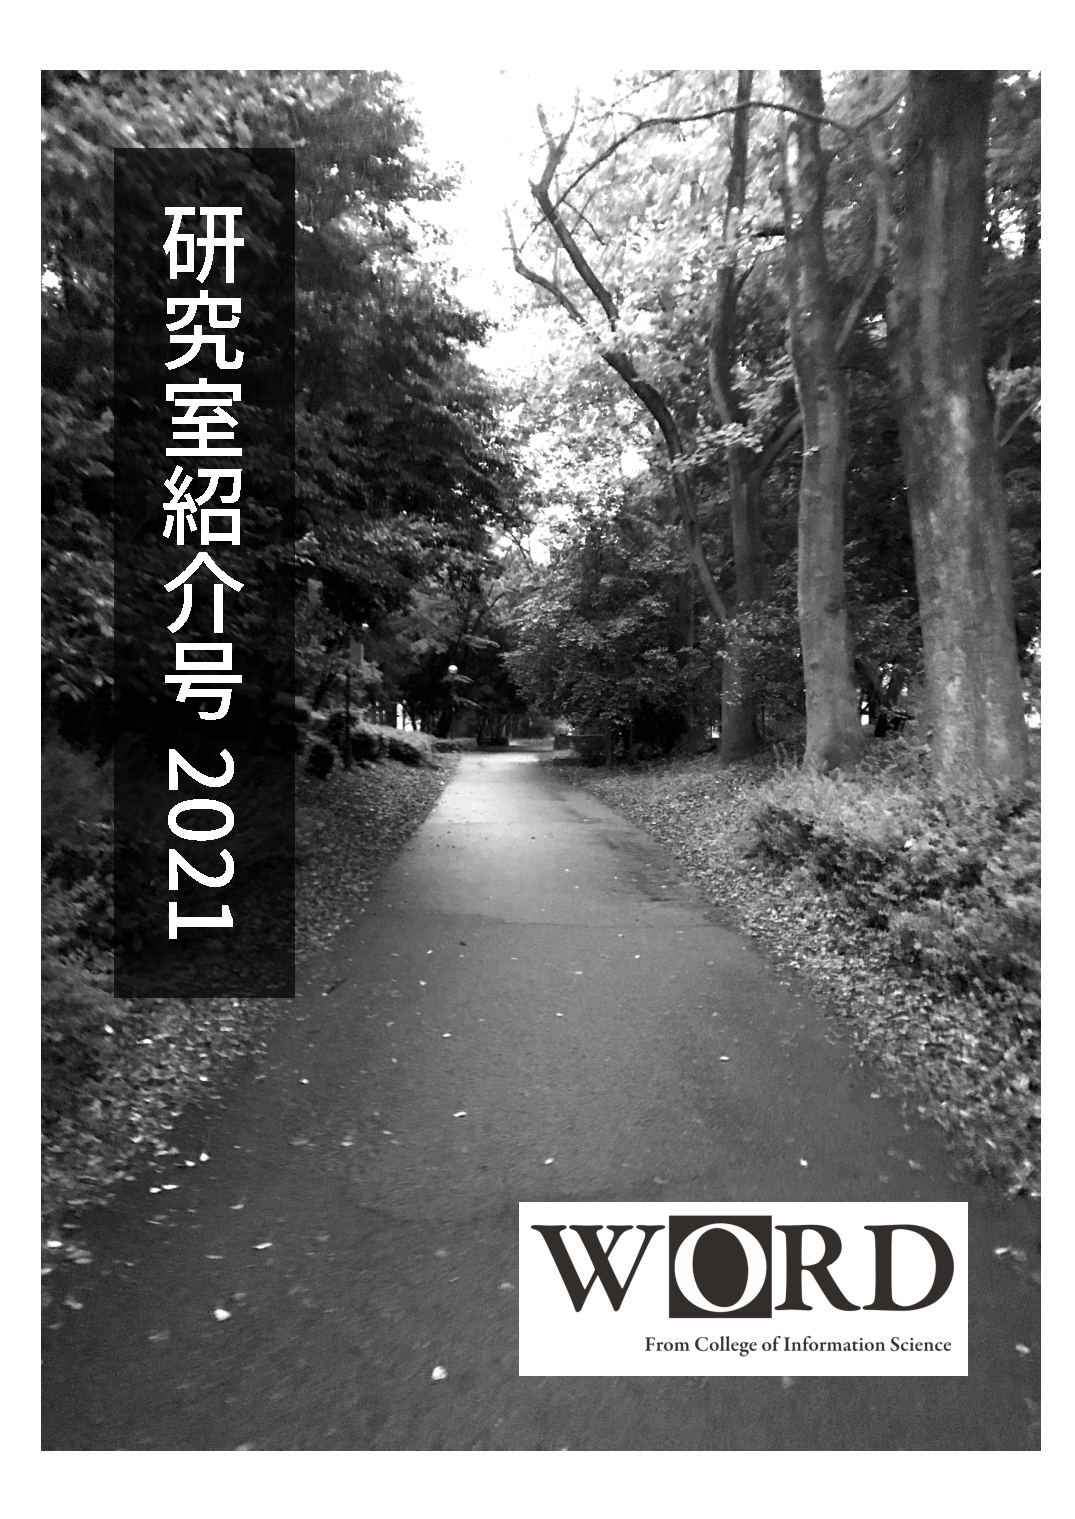
\includegraphics[width=32mm]{img/lab2021.pdf}
  \includegraphics[width=32mm]{img/word51.pdf}
  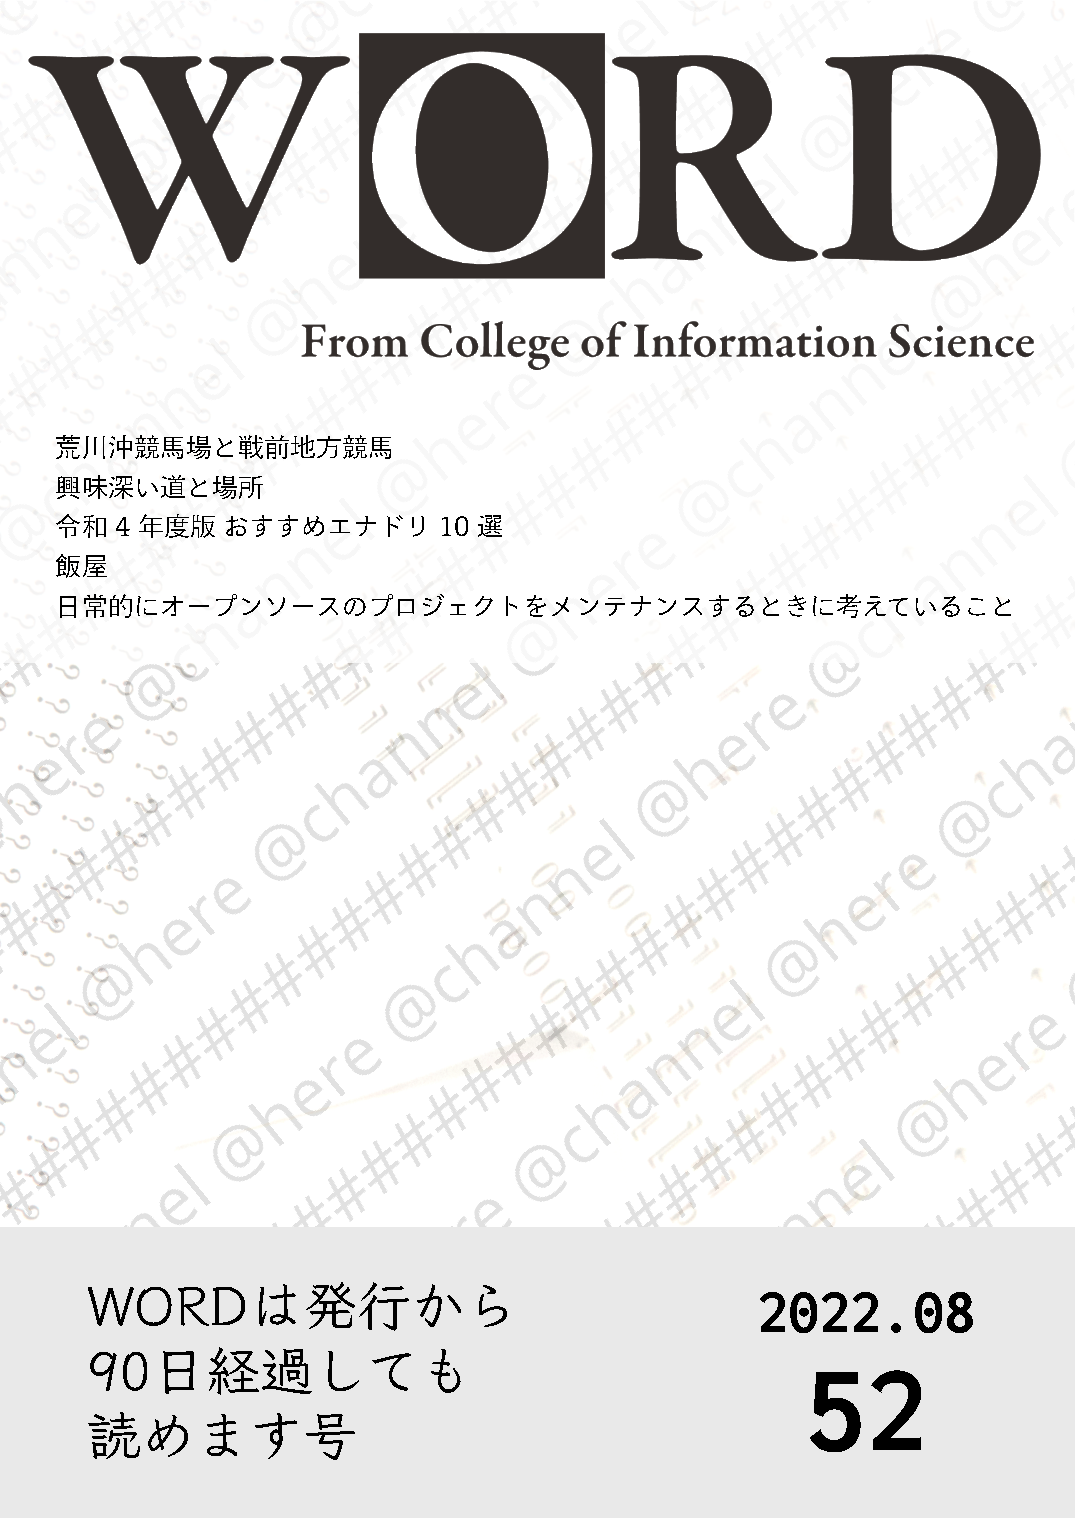
\includegraphics[width=32mm]{img/word52.pdf}
 \end{figure}
\end{frame}

\begin{frame}[plain]{『WORD』配布中!}

	本日「入学祝い号2023」を発行しました。
  1部ずつお持ち帰りください。

	普段は最新刊を3A・3C棟で配布しています。 お見かけの際はぜひ手にとってご覧ください。
\end{frame}

\begin{frame}[plain]{WORD編集部室(3C212)}
 \begin{itemize}
  \item 技術書の詰まった本棚
  \item 高速なインターネット環境とたくさんのパソコン・サーバ
  \item 24時間利用可能!
 \end{itemize}
  \begin{figure}
   \centering
   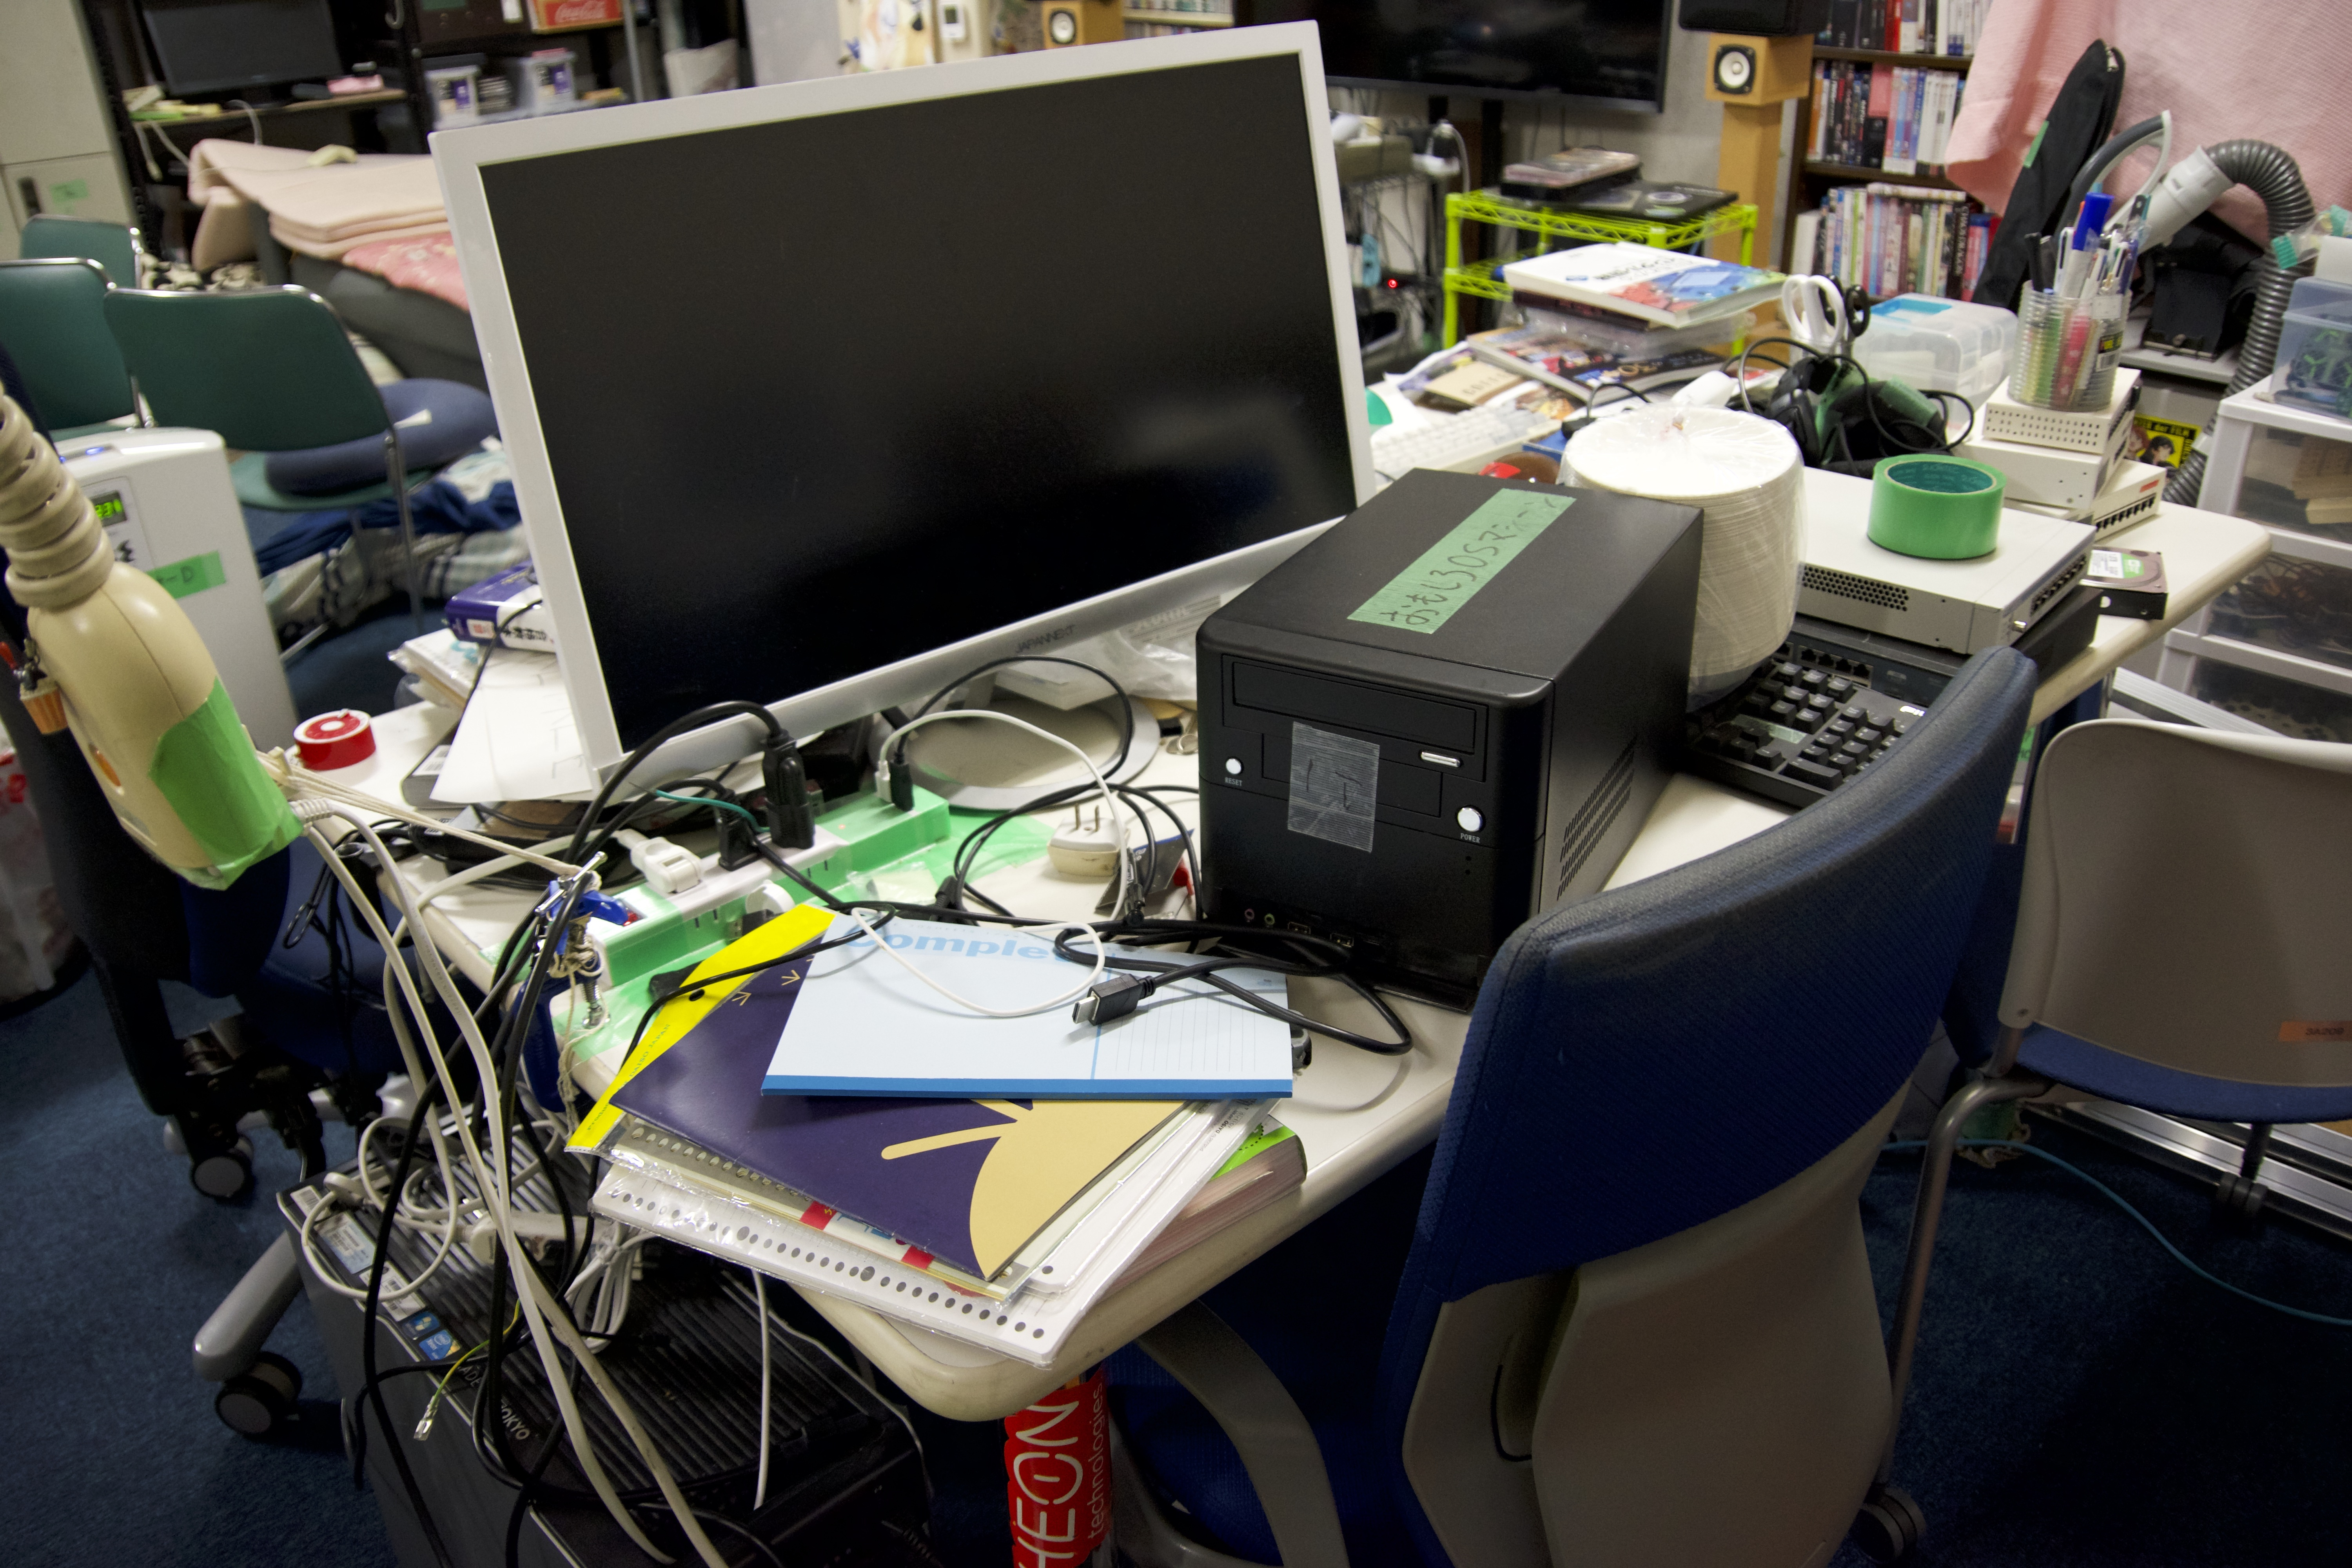
\includegraphics[width=50mm]{img/monitor.jpg}
   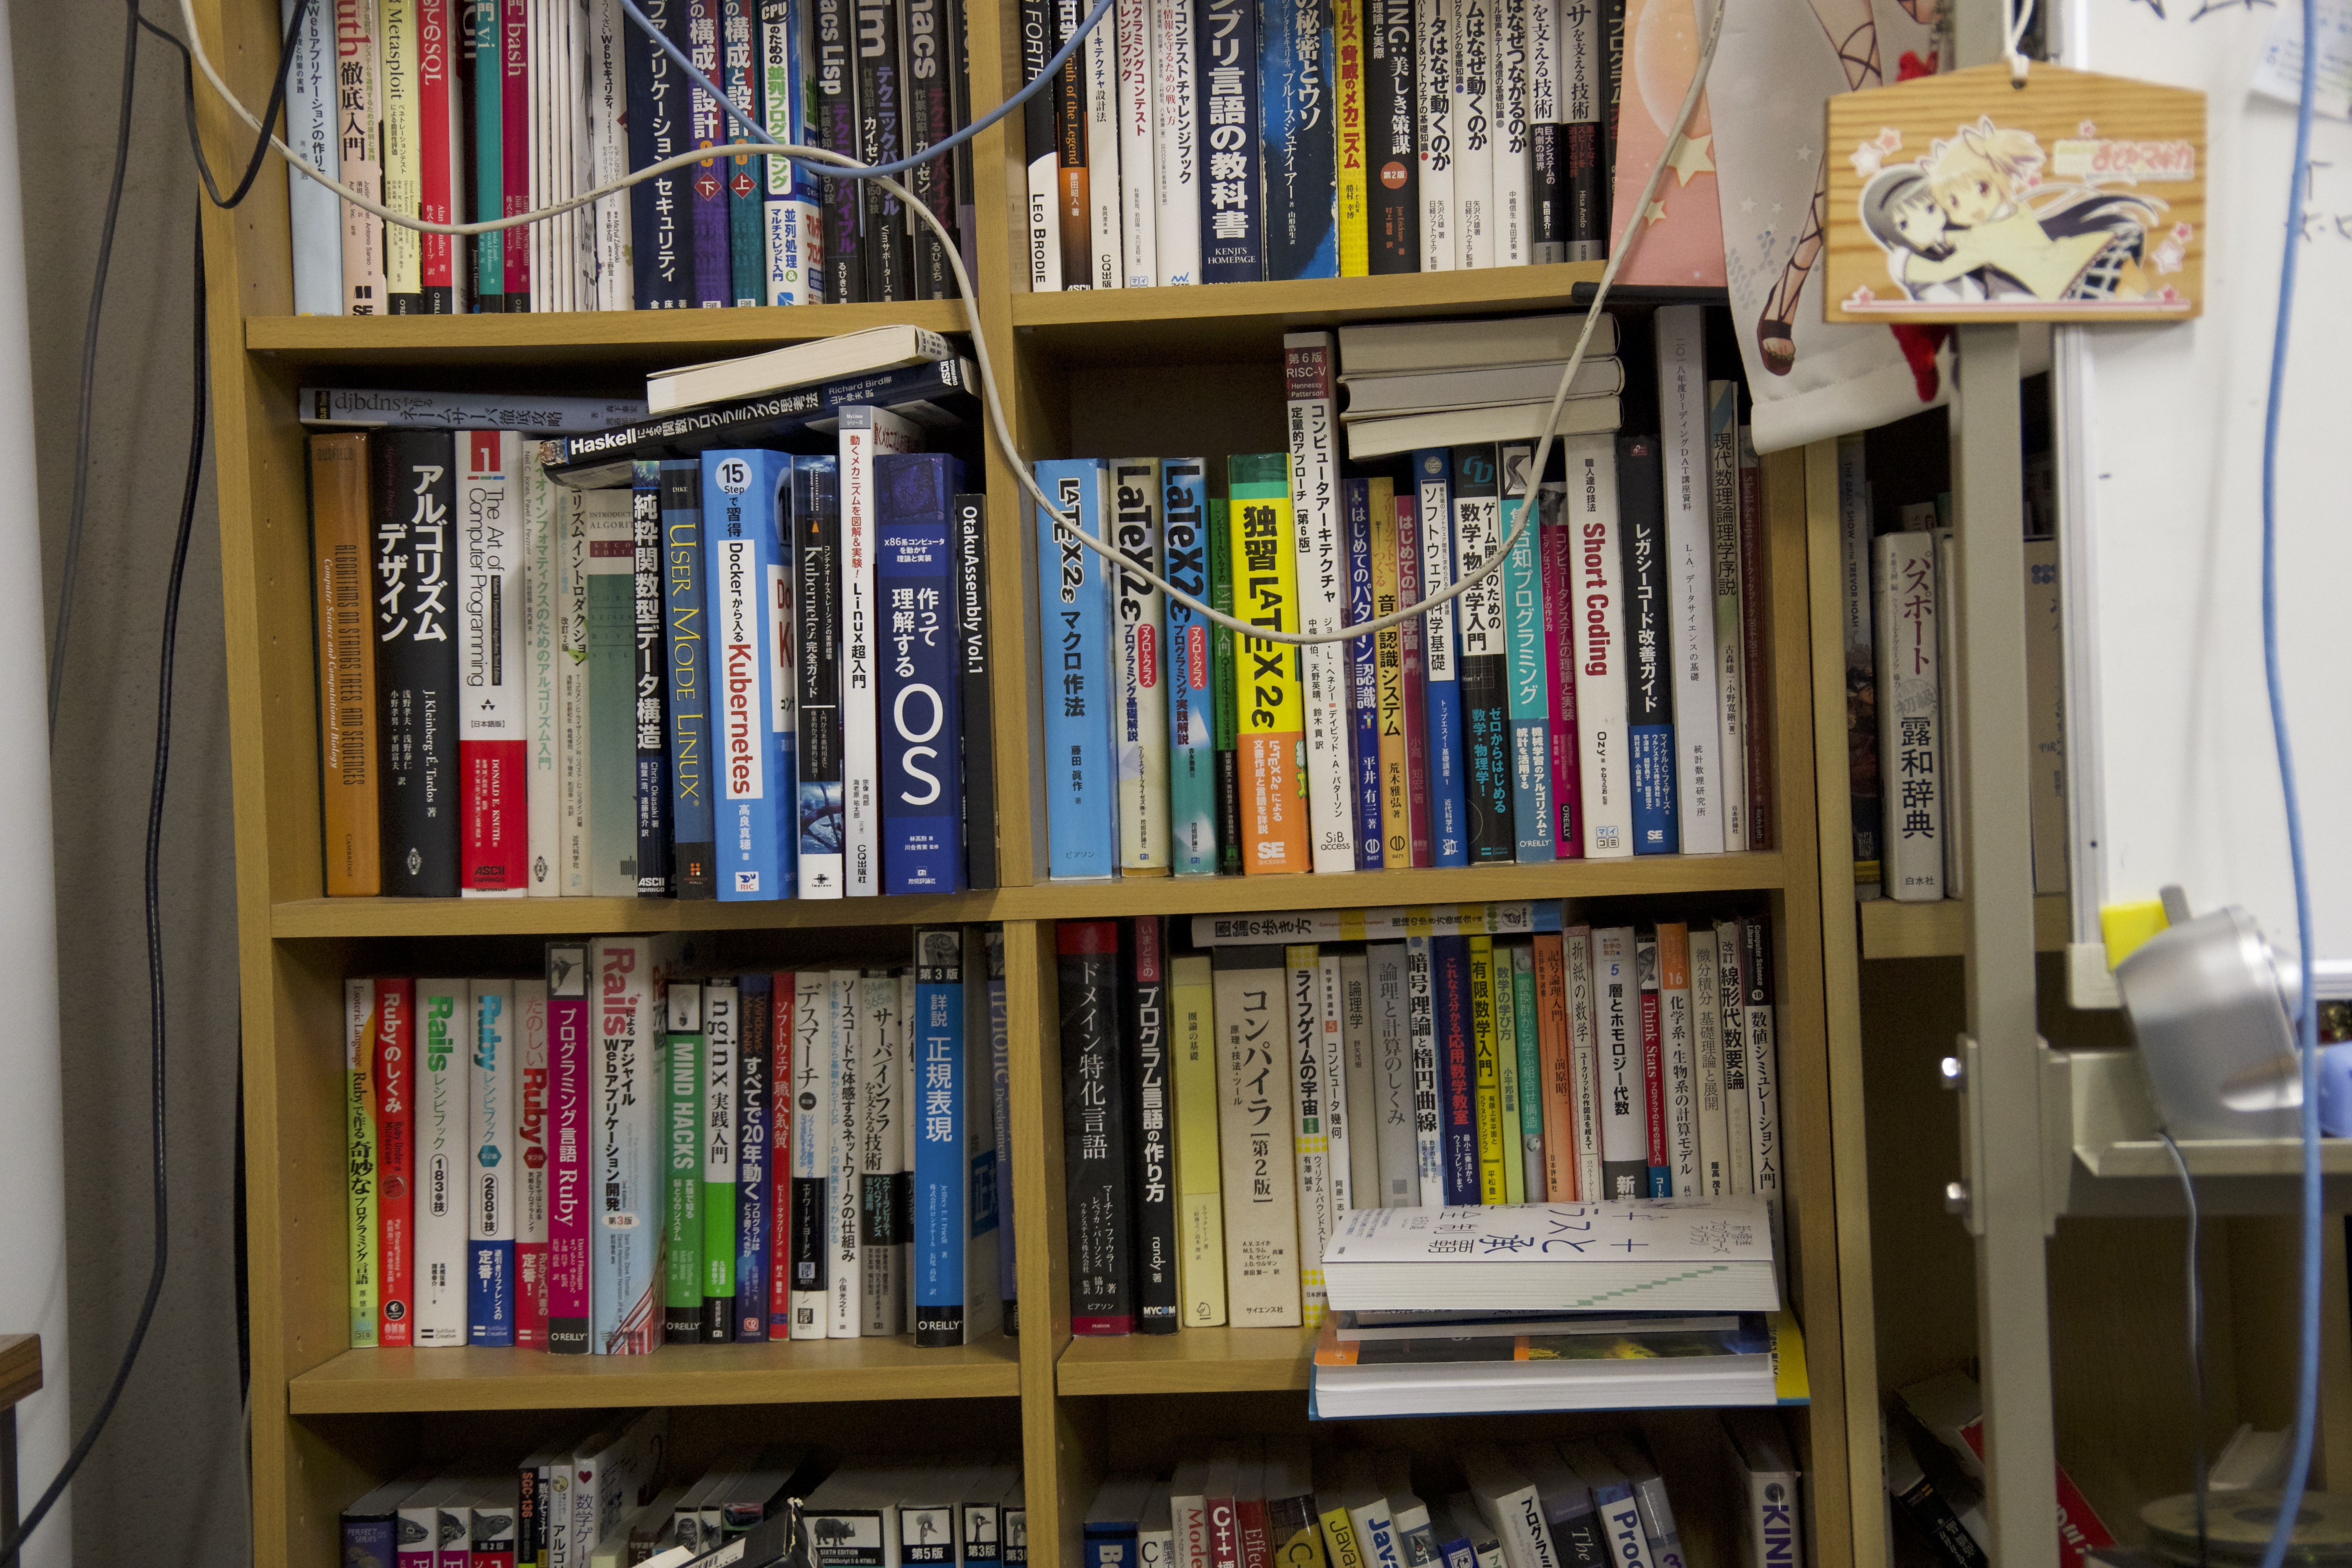
\includegraphics[width=50mm]{img/hondana.jpg}
  \end{figure}
\end{frame}

\begin{frame}[plain]{WORDに入るとできること}
  \begin{itemize}
   \item 編集部員としてWORD本誌に記事が書けます。
   \item 24時間編集室が利用できます。
   \item 編集室にある技術書や機材を自由に利用できます。
   \item 部屋のネットワーク・サーバーの管理ができます。
  \end{itemize}
\end{frame}

\begin{frame}[plain]{こんな人がいます}
 \begin{itemize}
  \item ネットワークやサーバに興味のある人
  \item (\LaTeX などの)組版に興味のある人
  \item 記事を書きたい人
  \item 自宅通学者で学内に居場所が欲しい人
 \end{itemize}
\end{frame}

\begin{frame}[plain]{よくある誤解:「WORDは技術強者しかいない」}
  \begin{itemize}
    \item 嘘です。技術強者もいますが、勉強中の人もいます。
    \item 確かに、WORD編集部には「技術者コミュニティ」としての側面はあります。
    \item 「技術に関するすごい記事」を書かなければいけないわけではありません。
    \item ただし、「一年に一本は何か記事を書く」ことを約束にしています。
  \end{itemize}
\end{frame}

\begin{frame}[plain]{あなたとWORDを盛り上げたい!} 
  \begin{center}
  「おもしろ活動」の一部が、COVID-19の影響で途絶えている

    { \Huge \textbf{盛り上がりを戻すには\\ 今年しかない! }}
  \end{center}
\end{frame}

\begin{frame}[plain]{WORDに興味が出てきたら}
  
  \begin{center}
  まずは編集部室にお越しください。
  \end{center}

  \begin{itemize}
     \item ドアがしまっている時は、インターホンを押してください。人がいれば対応します。
     \item Twitterやメールで連絡をいただくとより確実にご希望の時間に案内できます。
    \item 本日見学希望の方は、この後私にお声がけください。
  \end{itemize}
\end{frame}


\begin{frame}[plain]
 \begin{center}
  \Huge\textbf{WORD編集部は,\\皆様をお待ちして\\おります!}
 \end{center}
\end{frame}

\begin{frame}[plain]{リンク集}
 \begin{itemize}
  \item \url{https://www.word-ac.net/}
  \begin{itemize}
   \item 最近の過去号はここから見られる
   \item \url{gemini://gemini.word-ac.net/}もあるよ
  \end{itemize}
  \item \url{https://twitter.com/word\_tsukuba}
  \begin{itemize}
   \item 動いたり動かなかったりするTwitter
   \item DMは開いてます
  \end{itemize}
  \item \url{https://github.com/WORD-COINS}
  \begin{itemize}
   \item issueやPRなど歓迎
   \item このスライドもGitHubで管理しています\footnote{\url{https://github.com/WORD-COINS/opencampus-slide}}
  \end{itemize}
 \end{itemize}
\end{frame}
\begin{frame}[plain]
 \begin{center}
  質疑応答
 \end{center}
\end{frame}
\end{document}

